% Options for packages loaded elsewhere
\PassOptionsToPackage{unicode}{hyperref}
\PassOptionsToPackage{hyphens}{url}
\PassOptionsToPackage{dvipsnames,svgnames,x11names}{xcolor}
%
\documentclass[
  12pt,
]{article}
\usepackage{amsmath,amssymb}
\usepackage{lmodern}
\usepackage{iftex}
\ifPDFTeX
  \usepackage[T1]{fontenc}
  \usepackage[utf8]{inputenc}
  \usepackage{textcomp} % provide euro and other symbols
\else % if luatex or xetex
  \usepackage{unicode-math}
  \defaultfontfeatures{Scale=MatchLowercase}
  \defaultfontfeatures[\rmfamily]{Ligatures=TeX,Scale=1}
\fi
% Use upquote if available, for straight quotes in verbatim environments
\IfFileExists{upquote.sty}{\usepackage{upquote}}{}
\IfFileExists{microtype.sty}{% use microtype if available
  \usepackage[]{microtype}
  \UseMicrotypeSet[protrusion]{basicmath} % disable protrusion for tt fonts
}{}
\makeatletter
\@ifundefined{KOMAClassName}{% if non-KOMA class
  \IfFileExists{parskip.sty}{%
    \usepackage{parskip}
  }{% else
    \setlength{\parindent}{0pt}
    \setlength{\parskip}{6pt plus 2pt minus 1pt}}
}{% if KOMA class
  \KOMAoptions{parskip=half}}
\makeatother
\usepackage{xcolor}
\usepackage[margin=1in]{geometry}
\usepackage{graphicx}
\makeatletter
\def\maxwidth{\ifdim\Gin@nat@width>\linewidth\linewidth\else\Gin@nat@width\fi}
\def\maxheight{\ifdim\Gin@nat@height>\textheight\textheight\else\Gin@nat@height\fi}
\makeatother
% Scale images if necessary, so that they will not overflow the page
% margins by default, and it is still possible to overwrite the defaults
% using explicit options in \includegraphics[width, height, ...]{}
\setkeys{Gin}{width=\maxwidth,height=\maxheight,keepaspectratio}
% Set default figure placement to htbp
\makeatletter
\def\fps@figure{htbp}
\makeatother
\setlength{\emergencystretch}{3em} % prevent overfull lines
\providecommand{\tightlist}{%
  \setlength{\itemsep}{0pt}\setlength{\parskip}{0pt}}
\setcounter{secnumdepth}{-\maxdimen} % remove section numbering
\usepackage{longtable}
\usepackage{graphics}
\usepackage{xparse}
\usepackage{moresize}
\usepackage{setspace}
\usepackage{tcolorbox}
\usepackage{wrapfig}
\usepackage{helvet}
\usepackage{sectsty}
\usepackage{fancyhdr}
\usepackage{xpatch}
\usepackage{booktabs}
\onehalfspacing
\pagestyle{fancy}
\definecolor{gssmidblue}{RGB}{32, 115, 188}
\definecolor{dfeheadingblue}{RGB}{16, 79, 117}
\renewcommand{\familydefault}{\sfdefault}
\allsectionsfont{\color{dfeheadingblue}}
\sectionfont{\color{dfeheadingblue}\fontsize{16}{18}\selectfont}
\fancyhead[C]{}
\fancyhead[RL]{}
\fancyfoot[LR]{}
\fancyfoot[C]{\sffamily \thepage}
\renewcommand{\headrulewidth}{0pt}
\renewcommand{\footrulewidth}{0pt}
\futurelet\TMPfootrule\def\footrule{{\color{gssmidblue}\TMPfootrule}}
\usepackage{floatrow}
\floatsetup[figure]{capposition=top}
\usepackage[tableposition=top]{caption}
\usepackage[titles]{tocloft}
\renewcommand{\cftdot}{}
\AtBeginDocument{\let\maketitle\relax}
\usepackage{cellspace}
\usepackage{etoolbox}
\colorlet{headercolour}{DarkSeaGreen}
\ifLuaTeX
  \usepackage{selnolig}  % disable illegal ligatures
\fi
\IfFileExists{bookmark.sty}{\usepackage{bookmark}}{\usepackage{hyperref}}
\IfFileExists{xurl.sty}{\usepackage{xurl}}{} % add URL line breaks if available
\urlstyle{same} % disable monospaced font for URLs
\hypersetup{
  pdftitle={workshop\_R},
  pdfauthor={Department for Education},
  colorlinks=true,
  linkcolor={Maroon},
  filecolor={Maroon},
  citecolor={Blue},
  urlcolor={blue},
  pdfcreator={LaTeX via pandoc}}

\title{workshop\_R}
\author{Department for Education}
\date{}

\begin{document}
\maketitle

\resizebox{48mm}{!}{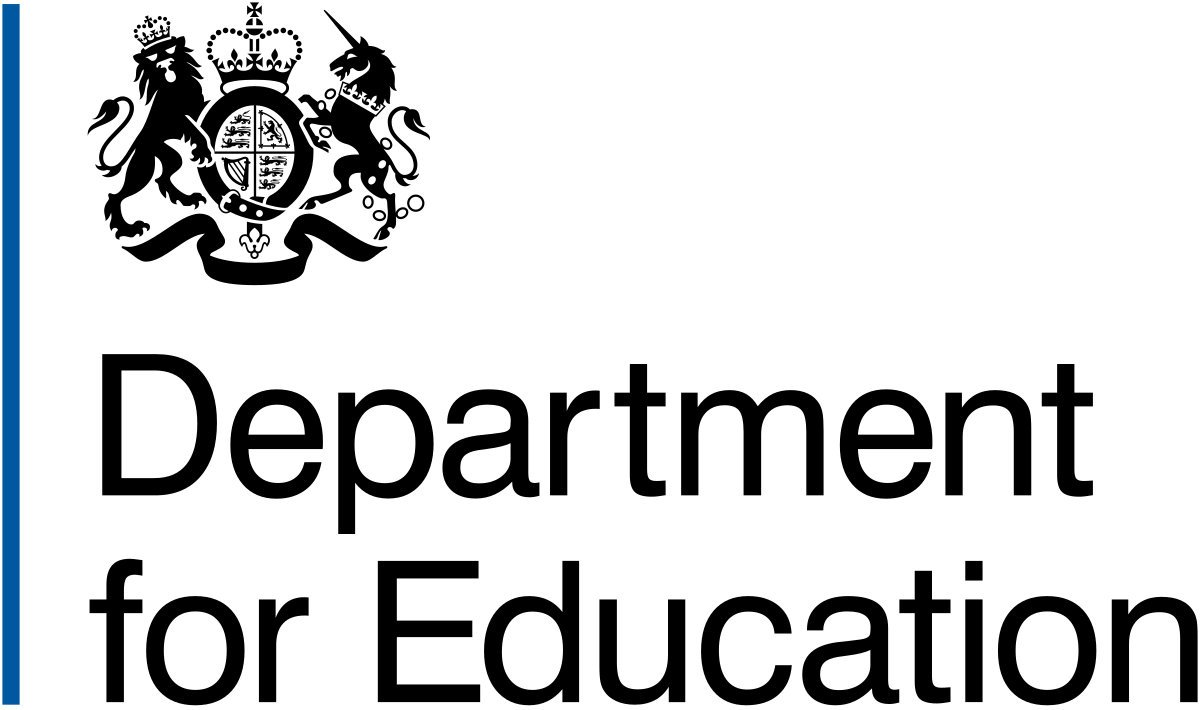
\includegraphics{images/Department_for_Education.png}}

\vspace*{0.24\textheight}

\raggedright\HUGE{\color{dfeheadingblue}\textbf{DfE Statistics Development Team Workshops}} 

\huge{\color{dfeheadingblue}\textbf{Coding RAP using R}}
\vspace*{2\baselineskip} 

\normalsize 
 \newpage 


{
\hypersetup{linkcolor=}
\setcounter{tocdepth}{2}
\tableofcontents
}
\newpage

\hypertarget{introduction}{%
\section{Introduction}\label{introduction}}

We've prepared this walkthrough guide for statistics publication teams
as an introduction to the ways in which coding in R can be used for
Reproducible Analystical Pipelines (RAPs), creating functions for
typical tasks that teams may come across. The guide is intended to be
step-by-step, building up from the very basics. The plan is to work
through this in groups of 3-ish with access to experienced R users for
support. If it starts too basic for your level, then just go through at
your own/your group's pace as you see fit. By no means can we cover
everything in this walkthrough, so please see it as a prompt to ask
follow-up questions as you're working through on anything related to R,
RAP and coding in general.

\hypertarget{what-is-a-rap}{%
\subsection{What is a RAP?}\label{what-is-a-rap}}

RAP stands for Reproducible Analytical Pipeline. The full words still
hide the true meaning behind buzzwords and jargon though. What it
actually means is using automation to our advantage when analysing data,
and this is as simple as writing code such as an R script that we can
click a button to execute and do the job for us.

Using R (the coding language) really helps us to put the R in RAP
(`reproducible'). Ask yourself, if someone else picked up your work,
could they easily reproduce your exact outputs? And when the time comes
around to update your analysis with new data, how easy is it for you to
reproduce the analysis you need? In an ideal RAP, it would be as simple
as plugging the new data in and clicking `go', with no need to manually
scroll through multiple scripts updating the year in every file name or
the variable name that's changed from using \_ to -.

\hypertarget{what-is-rr-studio}{%
\subsection{What is R/R Studio?}\label{what-is-rr-studio}}

R is a coding language. There are many different languages of code, some
others include SQL, python, JavaScript and many more. They all have
benefits, and the difference is often the syntax used (literally like
learning new languages!). R is open-source, meaning it is free, anyone
can use it and anyone can contribute to developing new `packages'.

\begin{itemize}
\item
  A \emph{package} is a set of functions someone else has written and
  tied together in a nice neat bow, ready for you to use! You simply
  install the package, and then you have all of the functions available.
\item
  A \emph{function} is a chunk of code that has been grouped together,
  given a name, and often has `place holders' you can change, such that
  you can use that name to run that code, and apply it to different
  data. For example, mean(x) is a function that calculates the
  arithmetic mean of x. You replace x with any numeric data.
\end{itemize}

R Studio is a piece of software, specifically an integrated development
environment (IDE), that enables us to write code in the R coding
language, while also providing a visual and interactive interface. It
has useful areas and windows that enable you to see what tables you have
loaded, charts you have created, Git user interface, file explorer, help
windows and many more! Normally you will see the screen split into 3 or
4 windows:

\begin{figure}
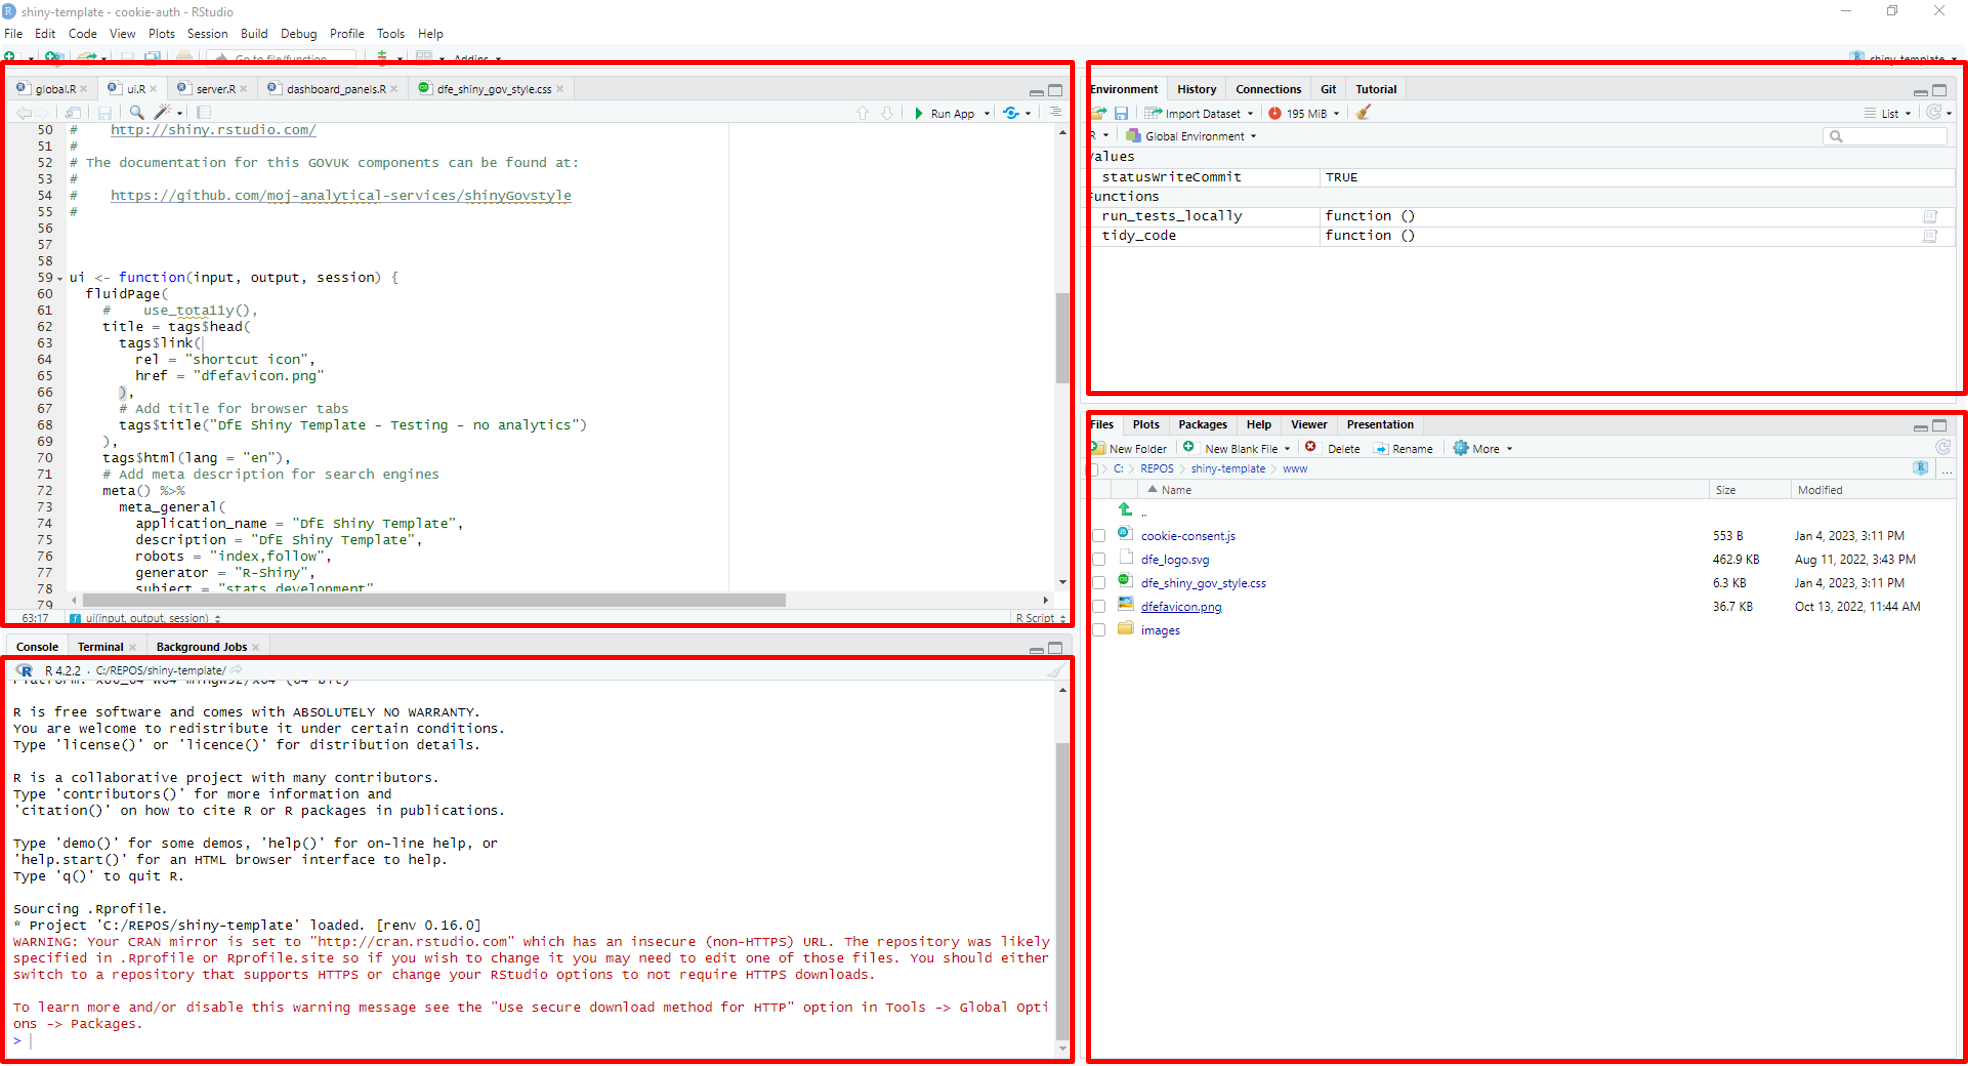
\includegraphics[width=1\linewidth]{images/RforRAP/R-studio-panels} \caption{R studio panels}\label{fig:unnamed-chunk-1}
\end{figure}

\begin{itemize}
\item
  Top left - Source pane. Open and view your code scripts, tables, data
  sets, functions.
\item
  top right - Environment/History/Connections/Git (if you have it). The
  environment shows you what data, functions, objects etc you have.
\item
  Bottom left - Console. Shows what you have run, and you can type and
  run commands directly into the console.
\item
  Bottom right - File explorer/plots/packages/Viewer.
\end{itemize}

\hypertarget{pre-workshop-requirements}{%
\section{Pre-workshop requirements}\label{pre-workshop-requirements}}

\hypertarget{technical-requirements}{%
\subsection{Technical requirements}\label{technical-requirements}}

First of all, make sure to bring your laptop. This is going to be
interactive and require you to do some coding.

Preferably before coming along, you'll need to go through the following
list of things you'll need to make sure are set up on your DfE laptop:

\begin{itemize}
\item
  Set up an Azure Dev Ops Basic account (not a Stakeholder account) at
  the DfE Service Portal; Either:
\item
  Install git on your laptop: \url{https://git-scm.com/downloads};
\item
  Install R-Studio on your machine: Download \textbf{R for Windows
  (x64)} and \textbf{RStudio} from the Software Centre on your DfE
  laptop.
\end{itemize}

Or:

\begin{itemize}
\tightlist
\item
  If you're on EDAP and used to using R/R-Studio and/or git on there,
  feel free to just use that.
\end{itemize}

You'll also need to make sure that git is set up in the git/SVN pane of
global options in R-Studio (found in the Tools drop down menu). Make
sure the path to your git executable is entered in the git path box and
git should automatically be integrated with R-Studio.

\begin{figure}
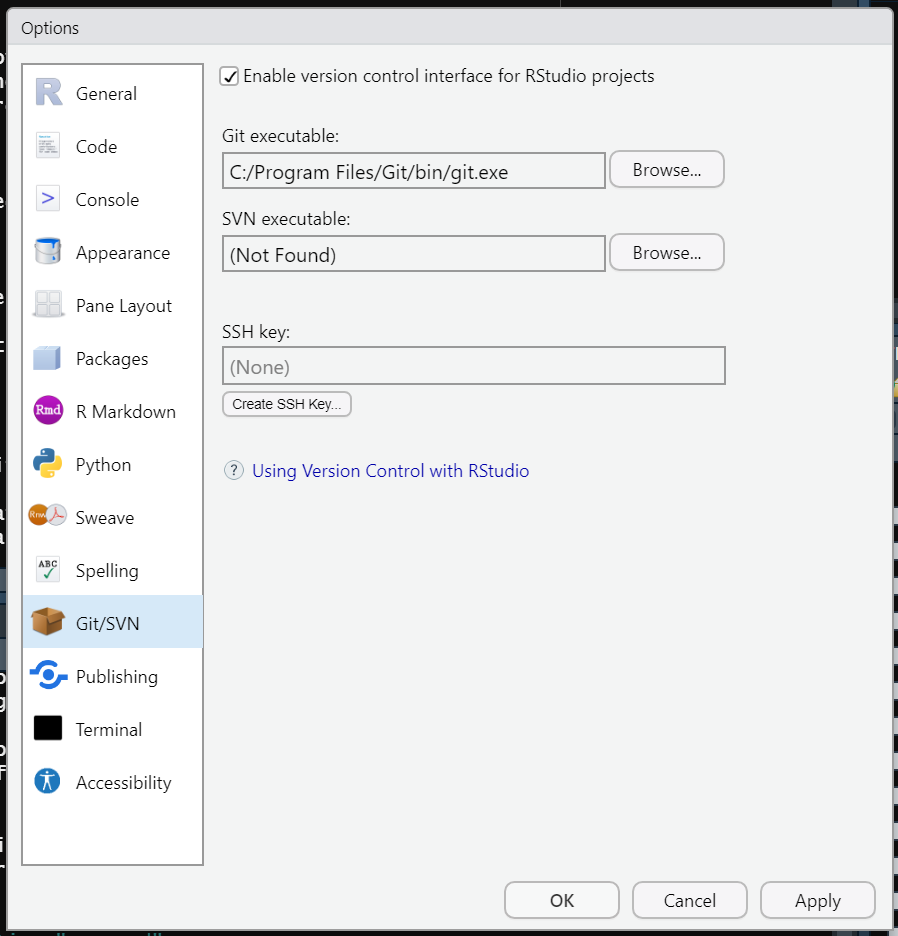
\includegraphics[width=0.64\linewidth]{images/gitdemo/gitdemo-gitRstudio-settings} \caption{Enter the path to your git executable in the git path option box}\label{fig:unnamed-chunk-2}
\end{figure}

Once you open a repository, you'll get an extra panel, named `git', in
the top right pane of R-Studio and you'll also be able to use git in the
`Terminal' tab at the bottom left (in the same place as the R console).

\begin{figure}
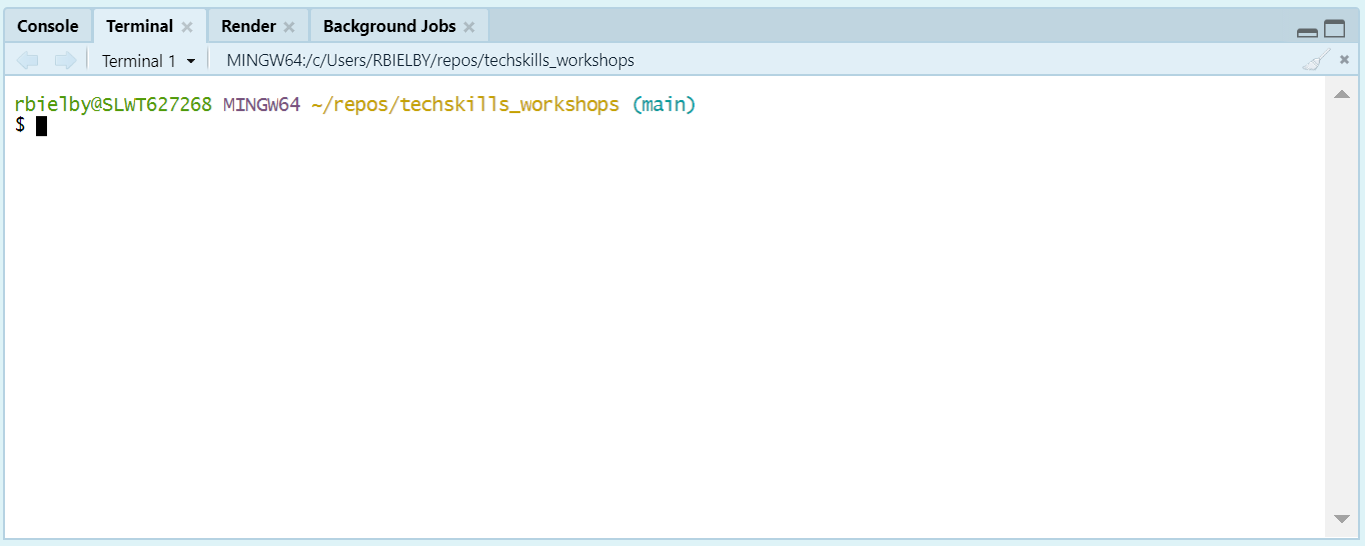
\includegraphics[width=0.56\linewidth]{images/gitdemo/gitdemo-gitRstudio-NewTerminal} \caption{The `git BASH` terminal in R-Studio}\label{fig:unnamed-chunk-3}
\end{figure}

A useful thing here if you want to use git commands in the terminal is
to switch the terminal from the default Windows Command Prompt to
\texttt{git\ BASH}. You can do this in the Terminal tab of R-Studio's
global options - just select \texttt{git\ BASH} from the `New terminal
opens with' pull down menu. Click apply and then select the Terminal tab
(next to the Console tab), click `Terminal 1' and then select `New
terminal' from the drop down menu. You should see something similar to
the terminal screenshot.

\hypertarget{working-in-groups}{%
\subsection{Working in groups}\label{working-in-groups}}

To get the most out of the workshop, we expect everyone to work through
all of the tasks themselves while discussing the work in small groups.
If anything is unclear then ask and most importantly, communicate with
each other about what you're doing.

So that we all have a record of what we have done, everyone will be
working in the same repository on their own branch. Once you have cloned
the repository, please \textbf{create a branch} called your name
(i.e.~\texttt{\textless{}firstname\textgreater{}\_\textless{}lastname\textgreater{}}).

By the end, you should get a good idea of how to utilize R for RAP
processes, as well as a brief understanding of using git.

\newpage

\hypertarget{getting-started}{%
\section{Getting started \ldots{}}\label{getting-started}}

Now we will begin the tasks and group work. First, everyone \textbf{open
up R studio.}

\hypertarget{creating-a-project-cloning-repositories}{%
\section{Creating a project \& cloning
repositories}\label{creating-a-project-cloning-repositories}}

When creating RAP processes, it's key that your code is reusable,
transparent, and well documented, such that it is future-proofed for any
future team members. Therefore, first, we will show you how to create an
R project. Using an R project ensures that all of the files in the
project folder (scripts, plots, notes, etc.) can all be referenced
relative to the \textbf{.Rproj file} location. Basically, it removes the
need to set and get your working directory, and removes the need to use
long \& complete file paths. Instead, you essentially start any file
path from the location of the .Rproj file! \emph{For example}, if you
have a code.R code script, and a data.csv file in a project folder that
has been set up as an R project, and you want to read the .csv in the R
script, you don't need the entire file path of the csv (which probably
starts C:/\ldots{} and can get very long), just the file path relative
to the \emph{.Rproj file} which in this case would simply be `data.csv'.

If you're struggling to grasp that, that's okay, we will create a
project and see this in action today. To create a new project, in R
studio, go to \textbf{File \textgreater{} New Project \textgreater{}
\ldots{}}. If you were creating a new R project that was not linked to
an online \emph{Git} repository, you would select \textbf{File
\textgreater{} New Project \textgreater{} New directory \textgreater{}
New Project}, \emph{however}, today we will be using
\href{https://github.com/dfe-analytical-services/techskills_workshops}{the
GitHub repository for the workshop}. Using Git repositories is best RAP
practice as it means you're using version control software and your work
is more easily shared transparently within your team/department.
Therefore, today we will select \textbf{File \textgreater{} New Project
\textgreater{} Version Control \textgreater{} Git}. To get the
repository URL, go to the GitHub repository, click the green `code'
button and copy the link from there. You can choose the project
directory name, as this is how it will appear on your device.

For the file path at the bottom, you should make sure this is
\textbf{not} saved in your OneDrive area. You should select Browse and
navigate out of OneDrive to save the project directory elsewhere (this
is because OneDrive has it's own version-control system, and trying to
use Git within that can cause complications and errors).

\textbackslash makebox{[}1.00\linewidth{]}\{ \centering

\begin{tcolorbox}[colback=gssmidblue, 
 leftright skip=0.1cm,
 coltext=white, 
 halign=left, 
 fontupper={\Huge \bfseries},
 fontlower={\large \bfseries},
 sharp corners, 
 colframe=gssmidblue,
 width=0.49\linewidth,
 boxrule=0pt,
 equal height group=introbox
 ]
Task
\tcblower
task info blah blah 
\end{tcolorbox}

Click `Create project'.

\hypertarget{using-renv}{%
\subsection{Using renv}\label{using-renv}}

Renv (short for R environment) is a package in R that helps you to keep
a record of which packages your project uses, and what version of each
package it should use (for a reminder of what a package is, check back
to the What is R/R Studio? section above). Using renv in your R project
means that anybody in the future (including your future self) who comes
back to this project, can immediately get all of the required packages.
First you need to install the renv package by running
\texttt{install.packages(\textquotesingle{}renv\textquotesingle{})} in
the console.

Once that has installed, you can run the functions from this package.
You can also see what packages are installed by navigating to the
`Packages' tab in the bottom right window - renv should have appeared in
here now.

When using functions from packages, you can either type
\texttt{\textless{}package\ name\textgreater{}::\textless{}function\ name\textgreater{}}
)(e.g.~\texttt{readr::read\_csv()}) or just the function name on its
own. However, problems can arise if two packages have different
functions with the same name. When you have loaded two packages that
contain functions with the same name and you only type the function
name, R automatically uses the function from the package that was loaded
most recently. If you want to choose which package to use and override
the precedent set by R, you should use the package name and colons to
explicitly state the source package and function you intended.

To activate renv, run \texttt{renv::activate()} in the console. If you
navigate back to the files tab in the bottom left and look in your
project folder, you should see some renv-related files have appeared,
including a \emph{renv.lock} file. The renv.lock file is the file that
records all of your project's packages and their versions. If you click
on the renv.lock file it will open for you to view in the top left.

Each time you add or remove packages, or update the package versions,
you should run \texttt{renv::snapshot()} to take a snapshot of the
current state of your library. If you ever get a new device, or someone
else wants to view your project, they simply need to run
\texttt{renv::restore()} to restore the package library on their device
to match the packages recorded in the renv.lock file.

\hypertarget{your-initial-script}{%
\section{Your initial script}\label{your-initial-script}}

Now that we have your project created and renv activated, we can create
our first code script. Open a new R script file by selecting
\textbf{File \textgreater{} New File \textgreater{} R script}.

\hypertarget{comments-and-headings}{%
\subsection{Comments and headings}\label{comments-and-headings}}

Comments in code are some of the most useful documentation you can use,
and are crucial for RAP! You should start your script with comments that
provide important information such as what this code script contains and
what it is for - basically anything you think a new person would need to
know in order to understand and run the code effectively. You add
comments in R scripts by starting the line with a \textbf{hash symbol,
\#}. Any line that starts with a hash symbol will be treated as a
comment rather than code, and so will not be `run'. You can also add
comments to the end of lines of code by including the hash symbol
half-way through a line - everything after the \# will be treated as a
comment, and everything before will be treated as code. If you have
multiple lines of comments you wish to add, you can type them out,
highlight them and use \texttt{ctrl+shift+C} to `comment out' all of the
highlighted lines.

Add some comments to the beginning of your script now - include your
name, the date, and a short description that explains that this is the
first script, and will include library calls as well as loading data and
any functions that will be used in future.

Your first script should definitely include the `library-calls' for all
of the packages you will need. This basically means loading any packages
you need at the beginning, before running any future code that requires
them. We load/call packages by using the \texttt{library()} function.

Our first steps only require two packages, `readr' and `dplyr'. You can
either install these by typing
\texttt{install.packages(\textquotesingle{}readr\textquotesingle{})} and
\texttt{install.packages(\textquotesingle{}dplyr\textquotesingle{})} one
at a time in the console, or you can install both packages at once by
running
\texttt{install.packages(c(\textquotesingle{}readr\textquotesingle{},\ \textquotesingle{}dplyr\textquotesingle{}))}.
Then, remember to take a \texttt{renv::snapshot()} to add these to the
renv.lock file!

Now, below your initial comments, we will add the library calls to the
script. First, we should add a section header! Section headers are yet
again another form of good documentation, and and extremely helpful when
navigating around scripts of code! To add a section header, we can use
the keyboard shortcut \texttt{ctrl+shift+R}. In the pop-up window, give
the first section the header `Load in packages'. Then click okay and you
should see the header has appeared in your code. In the bottom left of
the code window, you should see the section header has appeared, and if
you click on the name you can navigate to other sections when you have
built up your script further.

\begin{figure}
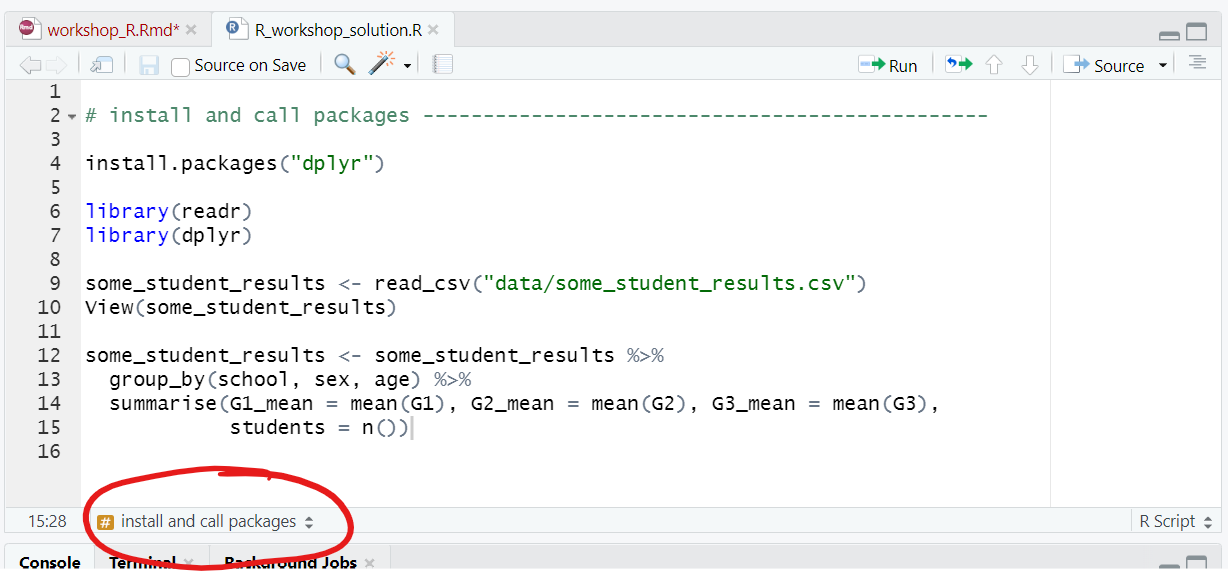
\includegraphics[width=1\linewidth]{images/RforRAP/section_headers} \caption{R Studio section headers navigation}\label{fig:unnamed-chunk-4}
\end{figure}

Another way to view and navigate between all of the sections in a script
is to use the keyboard shortcut \texttt{ctrl+shift+O} to open the
sections in a small panel on the right of your script.

Now save your initial script with the name `main.R'. You can save code
scripts by either selecting \textbf{File \textgreater{} Save As\ldots{}}
or by clicking the save icon in the bar below the script name. When your
script contains \textbf{unsaved changes}, the script name will turn red
and end with a * symbol. When it does not contain any unsaved changes,
the name of the script will turn black, with no * symbol, and the save
icon beneath it will grey-out.

\textbf{Throughout this workshop, make sure to add comments at every
step so you know what each code snippet is doing, and why!}

\hypertarget{adding-and-running-code}{%
\subsection{Adding and running code}\label{adding-and-running-code}}

Now, below the heading on a new line, add \texttt{library(readr)}, then
on a new line add \texttt{library(dplyr)}. In R, each new line
represents a new code command. You don't need to use a semi-colon or any
other punctuation to separate commands other than just starting a new
line, and you cannot have two commands on the same line. Therefore,
since the two library calls are two distinct commands because they load
different packages, they each need to be on a new line.

To actually run code that you have saved in a script file, there are a
few options. Firstly, there are buttons you can use to the top right of
the script file's window.

\begin{figure}
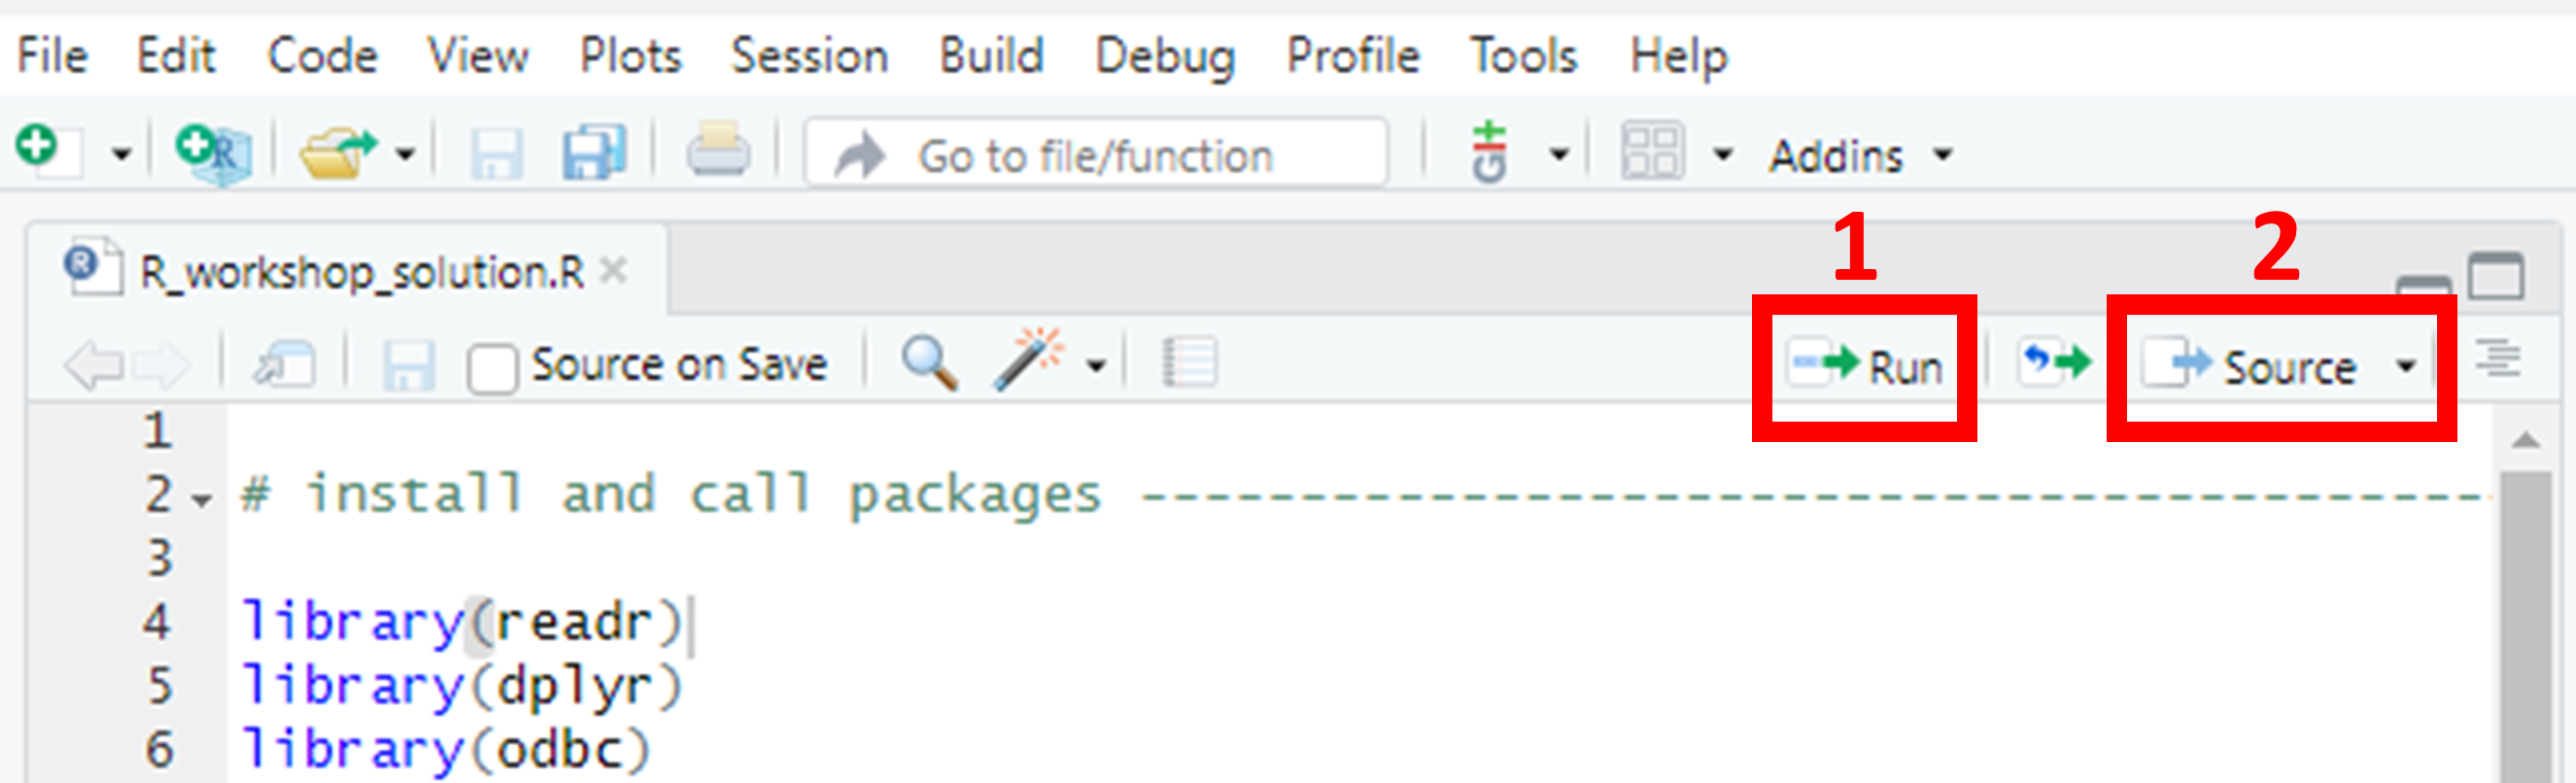
\includegraphics[width=1\linewidth]{images/RforRAP/run_buttons} \caption{R Studio run and source buttons}\label{fig:unnamed-chunk-5}
\end{figure}

Button 1 in the above image (the `run' button) will run either all
\emph{highlighted} code, or, if no lines are highlighted it will run the
line or snippet where your cursor is located (in the above image, you
can see the faint cursor line at the end of line 4, so clicking run
would run line 4 in this instance). Another way to do this is to use the
`run' keyboard shortcut - \texttt{ctrl\ +\ Enter}. This works in the
same way and will either run all highlighted lines, or the snippet where
the cursor is located.

Button 2 (the `Source' button) will run the entire script from the first
to the last line in one go! This is the same as running
\texttt{Source("script\_name.R")} in the console. \texttt{Source(...)}
is particularly useful in RAPs, as one of the baseline expectations for
statistics publication pipelines is that you have one script that runs
every single step of the process - sourcing scripts one by one in the
correct order in a `run\_pipeline' script (with comments!) is great way
to do this while keeping it tidy and clear!

Highlight the lines you have just added to the script and run them
either using the button or the keyboard shortcut. Now we have the
packages we need to load in some data.

\hypertarget{loading-in-the-data}{%
\subsection{Loading in the data}\label{loading-in-the-data}}

There are multiple ways to load data into R. Today we will cover two
common ways we see analysts use;

\begin{enumerate}
\def\labelenumi{\arabic{enumi}.}
\item
  Reading in a \textbf{CSV} file,
\item
  Loading data in directly from \textbf{SQL} servers.
\end{enumerate}

Before using either method to load in the data, we should add a new
section header! Use the guidance above to add a new section header
called `Load in the data'.

\hypertarget{reading-in-csvs}{%
\subsubsection{Reading in CSVs}\label{reading-in-csvs}}

We already installed the \texttt{readr} package, which contains the
functions we need to read CSVs into R. In R, it is best practice to name
our objects (tables, data sets, etc) so that you can use that name to
reference the objects you need. This means that while the code
\texttt{readr::read\_csv(insert\_filename/filepath\_here)} is the
function that reads in a given csv, we should write it in the below
format:

\texttt{chosen\_name\ \textless{}-\ readr::read\_csv(insert\_filename/filepath\_here)}

In this workshop, the data is available as a csv in the `data' folder of
the project, and is called \texttt{some\_student\_results.csv}.
Therefore, the code will look like this:

\texttt{student\_results\ \textless{}-\ read\_csv("data/some\_student\_results.csv")}

Write and run this line in your script. Then, if you navigate to the
`environment' window in the top right of the screen, you should see an
object has appeared with your chosen name under the heading `Data'. If
you click the blue circle with the white arrow inside, it will expand to
show you information about the data you've uploaded, including the name
of every column/variable, and the format of each column (i.e.~chr for
character, num for numeric). If you click the name of the object, it
will open in the viewer in the top left so that you can look at the
table. This is the same as typing \texttt{View(name\_of\_data)} in the
console.

\hypertarget{writing-to-and-reading-from-a-sql-database}{%
\subsubsection{Writing to and reading from a SQL
database}\label{writing-to-and-reading-from-a-sql-database}}

In order to read and write data from and to a SQL database, we need to
install the relevant packages and connect to the SQL database. Firstly,
we need to install the \texttt{odbc} and \texttt{DBI} packages. Try to
use the above guidance to;

\begin{enumerate}
\def\labelenumi{\alph{enumi}.}
\item
  Install the \texttt{odbc}, \texttt{DBI} and \texttt{dbplyr} packages,
\item
  Add the library calls to the correct section of the initial script,
\item
  Take a snapshot to update the renv.lock file.
\end{enumerate}

Once you have completed the above steps, we can use the new packages to
connect to the secure SQL database. We use the following code (inserting
the server and database we require) to create an object with the
connection. You can call it anything, but common practice is to call
this connection `con':

\begin{verbatim}
# Connect to SQL database
con <- DBI::dbConnect(odbc::odbc(),
    Driver = "{SQL Server Native Client 11.0}",
    Server = "...",
    Database = "...",
    Trusted_connection = "Yes"
  )
\end{verbatim}

{[}Note that this code will only work for you if you have access to the
specified server and database, so only users with existing access can
use this code in R to connect and pull in data! If someone without
access tried to run this code, they would get an error in the R
console.{]}

\hypertarget{writing-a-table-to-a-sql-database}{%
\paragraph{Writing a table to a SQL
database}\label{writing-a-table-to-a-sql-database}}

There are a number of functions available in R that can write a data
frame to a table on a SQL database. Here we'll use the
\texttt{dbWriteTable()} function with our students dataframe:

\texttt{dbWriteTable(con,\ \ Id(schema\ =\ "dbo",\ table\ =\ \textquotesingle{}sd\_sandbox\_student\_results\textquotesingle{}),\ student\_results)}

Note the first argument the function takes is the database connection
you've already created, the second is the table location that you want
to write to on that database and the third argument is the data frame
that you're sending to the database.

\hypertarget{reading-a-table-from-a-sql-database}{%
\paragraph{Reading a table from a SQL
database}\label{reading-a-table-from-a-sql-database}}

Now that we have the connection stored and named, we can use it to read
in a table from the database into R. There are multiple ways to do this
- in this workshop we will cover two of them.

\begin{enumerate}
\def\labelenumi{\arabic{enumi}.}
\item
  Use \texttt{dplyr::tbl(con,\ table\_name)},
\item
  Use
  \texttt{RODBC::sqlQuery(con,\ "SELECT\ *\ FROM\ {[}table\_name{]};")}.
\end{enumerate}

Option one above is a very concise and tidy way to read in data from SQL
tables, which (as long as you've added descriptive comments) will make
your code easy to read and understand. This option runs extremely
quickly because rather than storing the SQL table as a data table in R,
it stores a `live connection' to the table in SQL. You can type the name
of the `tbl' object in the console, and it will provide a preview of the
SQL table using the live connection. In the environment it will appear
as a list rather than a data table.

Option two is slightly longer to write and takes much longer to run, but
it does allow you to write SQL queries directly in R, so if you have
previous experience with SQL you may find this useful. You can edit and
customise the SQL query, meaning you have the option of selecting
specific columns and filtering at this stage, rather than reading in the
entire table. Just ensure that you write the table\_name exactly how you
would in SQL (including schemas).

Whichever option you choose, you need to choose what name you would like
this object to have in R once the table is read in. It is best practice
to make object names descriptive but concise. This means describing what
the table contains, but not including unnecessary and repetitive words
such as `table' in the name. The data we are using today contains data
on the characteristics and grades of some students, so we might choose
to call the table `students'. We assign the table this name by using the
\texttt{\textless{}-} symbols, so the full snippet should look something
like this:

\begin{verbatim}
# Read in student data from SQL
student_results <- tbl(con, 'dbo.sd_sandbox_student_results')
\end{verbatim}

Add this under an appropriate heading/comment to your initial script.
Then, if you navigate to the `environment' window in the top right of
the screen, you should see an object has appeared with your chosen name
under the heading `Data'. If you click the blue circle with the white
arrow inside, it will expand to show you information about the data
you've uploaded, including the name of every column/variable, and the
format of each column (i.e.~chr for character, num for numeric). If you
click the name of the object, it will open in the viewer in the top left
so that you can look at the table. This is the same as typing
\texttt{View(name\_of\_data)} in the console.

\hypertarget{manupilating-data}{%
\section{Manupilating data}\label{manupilating-data}}

Once you have pulled data into R studio and you can see it in your
environment, it is likely you want to manipulate it in some way. In this
workshop, we have pulled in data that contains one line per student, so
one common task is to aggregate data, and get it in the correct tidy
format for EES.

\hypertarget{aggregate-filter-data}{%
\subsection{Aggregate \& filter data}\label{aggregate-filter-data}}

Aggregating data is a common task analysts in in statistics publication
face. In the data we have loaded into R studio in this workshop, there
is currently one line per student, containing that students
characteristics and grades. We want to aggregate this by certain
characteristics and get the average grade for each aggregated group.
Firstly, it's possible that we might want to filter on certain variables
so that we only include certain students in our data.

To \textbf{filter} data, we can simply use the \texttt{filter()}
function from the \texttt{dplyr} package, which we have already
installed and loaded. Here we will also introduce the \textbf{pipe}
symbol - \texttt{\%\textgreater{}\%}. You can either type it out
\emph{or} use the keyboard shortcut \texttt{Ctrl\ +\ Shift\ +\ M} to
insert it! As said before, in R, a new line is read as a new command,
however, sometimes we might have long snippets of code that should all
be run as one command! The pipe symbol is used with \texttt{dplyr}
commands to join up multiple lines into one command, and the order does
matter!

In our environment, we should see the data we have loaded in with the
name we gave it - `student\_results'. If we want to filter this, we
would do so in the following format:

\begin{verbatim}
student_results %>%
filter(column_name == contraint, 
      column_name2 < constraint2, 
      column_name3 %in% c(list1, list2, list3))
\end{verbatim}

You can give this a go in the console without storing the results in the
environment by simply running the above without giving it a name like we
did when we read the data in. If you wanted to store your results, you
would add \texttt{name\ \textless{}-} at the start of the first line. In
today's workshop, we don't need to filter the data before we start
aggregating. The first thing we want to do is specify the variables we
want to group the data by. In this example we want to group by
\textbf{year, school, sex} and \textbf{age}. This is very easily done
using the \texttt{group\_by()} function as below:

\begin{verbatim}
student_results %>%
group_by(year, school, sex, age)
\end{verbatim}

However, the output from running the above code will look like it hasn't
changed, because it doesn't know how to aggregate the groups yet. We
define this using the \texttt{summarise()} function \emph{after} the
\texttt{group\_by()} function. In this workshop we will use two common
aggregations; averages and counts, however, this method can be applied
to all sorts of aggregation methods!

Today, we want to aggregate the data such that we have a row for every
group of year, school, sex and age, with the summary statistics being
the mean grades (G1, G2, G3) and the total count of students in each
row. To start with, we will lay out the code in an explicit form, before
we discuss how to convert it to best practice. Running the following
code in the console will give the output we want:

\begin{verbatim}
student_results %>%
  group_by(year, school, sex, age) %>%
  summarise(G1_mean = mean(G1), 
            G2_mean = mean(G2), 
            G3_mean = mean(G1),
            students = n())
\end{verbatim}

Within the \texttt{summarise} statement, it's defining 4 new columns.
\texttt{G1\_mean\ =\ mean(G1)} means that the new column called G1\_mean
will be the mean of the previous G1 column when grouped by the variables
defined in the \texttt{group\_by()} statement. \texttt{students\ =\ n()}
creates a new column named students, which contains the number of rows
that have been included in each group.

While the above code works, it can be written in many different ways,
and while in this example we are only creating 4 summary columns and
using 4 grouping variables, in real life this can get messy the more
columns and variables we add! Copying and pasting functions and lines
and changing the names each time is prone to mistakes. For example, did
any of you notice that \textbf{there is a mistake in the above code}? I
forgot to update the final mean, which should have been taking the mean
of the G3 column! However, in my haste of copying and pasting the same
thing 3 times, I only updated the name to G3\_mean, while forgetting I
also needed to edit what was in the mean() brackets.

In real life, mistakes like this are more common than you'd think! There
are best practices in writing our code that can help us to avoid
mistakes like this. If you're applying the same function to multiple
columns like we are with \texttt{mean()} above, we can use
\texttt{across()}. The \texttt{across()} function in R allows you to
apply one function across a list of columns, and also enables you to
specify the new column's names! We can therefore rewrite the above code
as below:

\begin{verbatim}
student_results %>%
  group_by(year, school, sex, age) %>%
  summarise(across(c(G1, G2, G3), mean, .names = "{.col}_mean"), 
            students = n())
\end{verbatim}

In the above, we have \emph{nested} an \texttt{across()} function inside
a \texttt{summarise()} function.
\texttt{across(c(G1,\ G2,\ G3),\ mean,\ .names\ =\ "\{.col\}\_mean")}
means apply the \texttt{mean()} function to G1, G2 and G3 one-by-one,
and set the new column name to be the original column name followed by
\texttt{\_mean}. In this instance it might not seem much simpler than
the first version, however using `across' can be extremely useful when
real-life examples have extremely large data sets! Lets store the above
results in our environment now and call them
\texttt{student\_results\_aggregated} using the following code:

\begin{verbatim}
student_results_aggregated <- student_results %>%
  group_by(year, school, sex, age) %>%
  summarise(across(c(G1, G2, G3), mean, .names = "{.col}_mean"), 
            students = n())
\end{verbatim}

\hypertarget{reorder-and-rename-columns}{%
\subsection{Reorder and rename
columns}\label{reorder-and-rename-columns}}

Something that some analysts might leave to the end or do manually in
excel is reorder and rename columns. However, even simple steps such as
these are prone to human error and can result in big mistakes! It also
means that your process isn't fully \textbf{automated} or
\textbf{reproducible}, since someone new to your project wouldn't know
from looking at it what you have done, and therefore wouldn't be able to
recreate it! To avoid this, it's always best to do these simple steps in
the code. It also makes your own code robust - if your code for analysis
expects columns to have certain names, to all be lower case, or to be in
a certain order, and they aren't, it will cause errors later down the
line!

First, a very useful function to use is \texttt{names()}. Try running
\texttt{names(student\_results)} and
\texttt{names(student\_results\_aggregated)} in the console. It should
return a list of all of the variable/column names in the specified
tables. You can also use this to compare the names of two data sets by
running
\texttt{names(student\_results)\ ==\ names(student\_results\_aggregated)}.
This will return a \texttt{TRUE/FALSE} list - you will see in this case,
the first 3 are \texttt{TRUE} - this is because the names of the first 3
columns are school, sex, age in both tables, however the rest differ.
This is useful when you are \emph{expecting} two tables to have the same
variable names, for example in an annual publication cycle, it is a good
idea to check that the variable names this year are the same as they
were last year before you start your analysis.

First, lets reorder the columns. I want the '\texttt{students} column to
appear \emph{before} the grade means. We can simply use the
\texttt{select()} function here, listing the columns in the order we
wish them to appear:

\begin{verbatim}
student_results_aggregated %>%
  select(year, school, sex, age, students, G1_mean, G2_mean, G3_mean)
\end{verbatim}

Now if we also wanted to rename columns, we can do it together in one
step by using another `pipe' (\texttt{\%\textgreater{}\%}). If there are
only a select number of columns you wish to rename, you would use
\texttt{rename} and specify as follows:

\begin{verbatim}
student_results_aggregated %>%
  select(year, school, sex, age, students, G1_mean, G2_mean, G3_mean) %>%
  rename(g1_mean = G1_mean, g2_mean = G2_mean, g3_mean = G3_mean)
\end{verbatim}

So when using \texttt{rename} as above, the order needed is
\texttt{desired\_name\ =\ original\_name}. As you can see above, all
this code does is convert the upper case G's to lower case, however, you
could rename each column to anything you like using this method. It's
best practice to stay consistent with the case you use, and in EES, we
expect all column names in `snake\_case'. Therefore, something you might
want to do is rename all of the columns to lower case. If your
rename-step is something like converting all columns to lower case, this
can be done in a more effective way, with less copying and pasting,
using \texttt{rename\_all()} and \texttt{tolower()} like this:

\begin{verbatim}
student_results_aggregated <- student_results_aggregated %>%
  select(year, school, sex, age, students, G1_mean, G2_mean, G3_mean) %>%
  rename_all(tolower)
\end{verbatim}

Since above, we have started the first line with
\texttt{student\_results\_aggregated\ \textless{}-}, this means it's
going to overwrite whatever was stored in the environment under that
name before! This \emph{can} be risky, since \texttt{select()} can also
be used to \textbf{drop} columns. If you left out any names from the
select line by accident, they would simply be dropped, so be careful if
you use the same name as the object from before this step! This can be
avoided by picking a different name, like
\texttt{student\_results\_aggregated\_reordered} for example. If you
\emph{did} make a mistake, and overwrote something by accident, you can
just re-run the code that made the original object before it was
overwritten.

\hypertarget{suppression-and-writing-functions}{%
\subsection{Suppression (and writing
functions)}\label{suppression-and-writing-functions}}

Another common task that analysts face is suppressing data. In this
section, we will write our own function that will do the primary
suppression step for us! We have already been using functions from
\emph{packages} throughout this workshop - everything in the format
\texttt{function\_name()} is a function that has already been written
for us - it takes whatever we put in the brackets, does things to it,
and creates an output. Here we will introduce writing our own!

\hypertarget{writing-functions}{%
\subsubsection{Writing functions}\label{writing-functions}}

The best way to introduce writing functions is by starting very simple
to understand the concept first, so let's practice here with some easy
examples. Open a \textbf{new R script} (file \textgreater{} New file
\textgreater{} R script) and call it `functions.R'. On the first line,
add some \textbf{comments} that explain this script is to practice
writing functions.

Firstly, we will write a simple function that adds two numbers together.
Give it a heading that describes this. On a new line, we will use the
following syntax to create our first function:

\begin{verbatim}
function_name <- function(inputs...){
function instructions...
}
\end{verbatim}

In our function, we want to add two numbers, so we want two inputs. We
can call them whatever we want, but you should choose something logical
that makes it easy to understand. Whatever names you choose for the
inputs in the \texttt{function(...)} bracket, you then use those names
as place-fillers in the instructions. Then, whenever the function is
used, it will carry the inputs through the instructions in the right
places. Here is an example:

\begin{verbatim}
add_together <- function(x,y){
x + y
}
\end{verbatim}

The above function takes two inputs, x and y, and adds them together. To
\emph{use} the function, you need to run the above code once to
\emph{create} it, then you can use it in the console. You should also
see it appear under `functions' in your environment! Once it's created,
you can use it in the console by running \texttt{add\_together(2,3)} as
an example, giving the output of 5 if it's been written correctly! You
can choose whatever numbers you like to replace x and y when using it in
the console as above.

Functions can also include character inputs as well as numeric! Another
example we will use here to practice is creating a function that outputs
a sentence. a simple way to output text in R is to use the
\texttt{paste()} function. Try creating a function called
`introduction\_text', that has \emph{two inputs} defined as `name' and
`age', and uses
\texttt{paste("Hi,\ my\ name\ is",\ name,\ "and\ my\ age\ is",\ age)} as
the \emph{function instruction}. Test it out! Do you see your sentence
appearing in the console?

\hypertarget{if-and-ifelse-statements}{%
\subsubsection{if() and ifelse()
statements}\label{if-and-ifelse-statements}}

\texttt{if()} and \texttt{ifelse()} statements work similarly to using
IF in excel formulas - they apply tests and perform actions based on the
outcome of the test. In the console, if you type a question mark
followed by a function name it will open the help page for that package!
Try it out here by typing \texttt{?ifelse} and read the help page to
understand the syntax.

The difference between \texttt{if()} and \texttt{ifelse()} is that
\texttt{ifelse()} statements perform one yes/no test - for example
\texttt{ifelse(age\ \textgreater{}=\ 16,\ \textquotesingle{}16+\textquotesingle{},\textquotesingle{}under\ 16\textquotesingle{})}
tests whether age is greater than or equal to 16. If it is, then it
outputs `16+'. If it is not, then it outputs `under 16'.

If statements are different to ifelse statements - they can have
multiple conditions and can be stacked. For example;

\begin{verbatim}
if(age >= 16){
'16+'
} else if(age < 12){
'under 12'
} else if(age >= 12 & age < 16){
'12 - 16'
} else NA
\end{verbatim}

Here there are 3 `tests' and 4 different outputs. The outputs are either
`16+', `12-16', `under 12' or NA. You can also have multiple conditions
in one \texttt{if()} statement using \emph{and} (\texttt{\&} symbol) or
\emph{or} (\texttt{\textbar{}} symbol) depending on what you need. For
example;

\begin{verbatim}
if(age >= 16 & sex = 'Female){
'16+ female'
}
\end{verbatim}

This test is finding instances where age is greater than or equal to 16
AND sex is female. We might want to use \emph{or} in cases like the
following example:

\begin{verbatim}
if(object == 'Bread | object == 'Fish'){
object <- 'Food'
}
\end{verbatim}

The above rewrites object by combining two different options (Bread or
Fish) into one `Food' category.

\hypertarget{function-for-suppression}{%
\subsubsection{Function for
suppression}\label{function-for-suppression}}

Now that we now how to write our own functions, we can write one to help
us suppress data. First of all, we can demonstrate the suppression using
functions from existing packages. Let's go back to our main.R script. At
this point we should still have \texttt{student\_results\_aggregated} in
our environment. We want to suppress any rows that have less than 5
students. One way to do this is shown below:

\begin{verbatim}
student_results_aggregated_suppressed <- student_results_aggregated %>%
  mutate(g1_mean = ifelse(students < 5, 'c', g1_mean),
         g2_mean = ifelse(students < 5, 'c', g2_mean),
         g3_mean = ifelse(students < 5, 'c', g3_mean),
         students = ifelse(students < 5, 'c', students)
         )
\end{verbatim}

The above code takes the mean grade columns and uses an
\texttt{ifelse()} statement \emph{within} a \texttt{mutate()} statement.
Here, it's saying for each of the mean columns, if the number of
students is less than 5, then replace the entry in that mean grade
column with a `c', if not, then keep what is already in the column. Note
that we \emph{have} to do the students column last, because once we add
`c' to any column it becomes a character variable rather than numeric.
Since the previous columns are based on the numeric value of the
students, we must order it so that these mutations occur first, while
the student column is still a numeric variable and therefore able to
apply the \texttt{students\ \textless{}\ 5} logic.

While the above code works, the same issues arise as in the previous
aggregation section where you can end up copying and pasting the same
line many times depending on the size of your real-life data sets! We
want to avoid this type of repetition where possible so that we reduce
the possibility of making mistakes (like forgetting to update every line
you have copied and pasted). So let's create a function to suppress
counts less than 5. With an appropriate comment to explain, add the
below to your functions.R script.

\begin{verbatim}
suppress_counts <- function(column, count) {
  ifelse(count < 5, 'c', column)
}
\end{verbatim}

The above function takes a column, and performs the \texttt{ifelse}
statement from the previous example. Once you have created the function
and can see it in your environment, you can rewrite the above example
like this:

\begin{verbatim}
student_results_aggregated_suppressed <- student_results_aggregated %>%
  mutate(g1_mean = suppress_counts(g1_mean, students),
         g2_mean = suppress_counts(g2_mean, students),
         g3_mean = suppress_counts(g3_mean, students),
         students = suppress_counts(students, students))
\end{verbatim}

However, this \emph{still} includes some repetition we would rather
avoid! therefore, we can take this one step further and make use of the
\texttt{dplyr::across()} function. The \texttt{across()} function allows
you to apply the same function to multiple columns - type
\texttt{?dplyr::across} in the console to view the help page and more
information.

We can rewrite the above in the following way:

\begin{verbatim}
student_results_aggregated_suppressed <- student_results_aggregated %>%
  mutate(across(c(g1_mean, g2_mean, g3_mean, students), 
          ~suppress_counts(. , students)))
\end{verbatim}

So, we've just written the same thing in 3 different ways! While all
three options produce the same output, the last example is the best for
RAP, as it is the most concise and requires the least repetition.

\hypertarget{adding-new-columns}{%
\subsection{Adding new columns}\label{adding-new-columns}}

Another common task that many analysts face is needing to add new
columns to their data sets. In DfE, often analysts will need to add the
required Explore Education Statistics (EES) columns formatted in the
correct way. Using the
\href{https://rsconnect/rsc/stats-production-guidance/ud.html\#Overview_of_EES_data_files}{online
guidance}, we can see that the following columns are required for EES:
time\_identifier, time\_period, geographic\_level, country\_code (or
geographic level equivalent), country\_name (or geographic level
equivalent).

When uploading data to EES, you should aim to include at least 3 years
of data in EES where it exists in light of recent accessibility
legislation. This example has 3 years of data, 2015, 2016, 2016.
However, the time\_identifier is not specified yet, and the year column
is not correctly formatted!

Let's assume in this instance the time\_identifier is \emph{academic
year}. We can easily add this column, and rename the existing year
column using the following code:

\begin{verbatim}
student_results_aggregated_suppressed_EES <- student_results_aggregated_suppressed %>%
  mutate(time_identifier = 'Academic year') %>%
  rename(time_period = year)
\end{verbatim}

We also want to add the required geography columns. In this case, we are
going to use the `school' column to get the required geography using
\texttt{case\_when()} within \texttt{mutate()}. Assume that the school
`GP' is in London, and the school `MS' is in East England, and we want a
\emph{regional} geographic level (so we need region\_name and
region\_code). We can use the following code:

\begin{verbatim}
student_results_aggregated_suppressed_EES <- student_results_aggregated_suppressed %>%
  mutate(time_identifier = 'Academic year', geographic_level = 'Regional',
         region_name = case_when(school == "MS" ~ "East of England",
                                 school == "GP" ~ "London")) %>%
  rename(time_period = year)
  
\end{verbatim}

The above code gets us the correct geographic level and region name, but
not region code. We can use a \emph{look-up table} to get the correct
code\ldots{}

\hypertarget{joins-joining-geographic-codes-via-lookup-tables}{%
\subsection{Joins \& joining geographic codes via lookup
tables}\label{joins-joining-geographic-codes-via-lookup-tables}}

The
\href{https://github.com/dfe-analytical-services}{dfe-analytical-services}
area on GitHub holds all publicly available code from DfE. The code
behind the \href{https://rsconnect/rsc/dfe-published-data-qa/}{EES data
screener} is available here, and
\href{https://github.com/dfe-analytical-services/dfe-published-data-qa}{the
screener repository} contains a
\href{https://github.com/dfe-analytical-services/dfe-published-data-qa/tree/master/data}{folder
full of geographic lookup tables}!

Today we will use the
\href{https://github.com/dfe-analytical-services/dfe-published-data-qa/blob/master/data/regions.csv}{regions.csv}
file from this folder. We can pull the csv directly from the repo using
the `raw' URL:
\url{https://raw.githubusercontent.com/dfe-analytical-services/dfe-published-data-qa/master/data/regions.csv}.
Using this also means if the CSV is updated on GitHub, when you run your
code it will automatically pull the latest version of the CSV! Adding
appropriate headings and comments, pull in this lookup table using the
following code:

\texttt{\#\ Pull\ in\ regions\ lookup\ table}

\texttt{regions\_URL\ \textless{}-}
``\url{https://raw.githubusercontent.com/dfe-analytical-services/dfe-published-data-qa/master/data/regions.csv}''

\texttt{regions\_lookup\ \textless{}-\ read.csv(regions\_URL)}

The lookup table should have appeared in the environment! Click on the
name to open it, or use the code \texttt{View(regions\_lookup)}. Now we
can join the codes to our data using the region name using the
\texttt{left\_join()} function! We can `pipe' joins in the exact same
way we have piped summarise, group\_by, mutate and rename statements. In
the console, type \texttt{?join} to see the different types of join
within the \texttt{dplyr} package!

Here we will use a left join because we want to keep all of the rows
from our data, and only join on rows that match from the lookup table.
We can use the following code to join the region code using region name
and reorder the columns:

\begin{verbatim}
student_results_aggregated_suppressed_EES <- student_results_aggregated_suppressed %>%
  mutate(time_identifier = 'Academic year', geographic_level = 'Regional',
         region_name = case_when(school == 'MS' ~ "East of England",
                                 school == 'GP' ~ 'London')) %>%
  rename(time_period = year) %>%
  left_join(regions_lookup, by = c('region_name' = 'region_name')) %>%
  select(time_period, time_identifier, geographic_level, region_name, 
         region_code, sex, age, students, g1_mean, g2_mean, g3_mean)
\end{verbatim}

The data created should now look a lot like what you would normally
upload to EES.

\hypertarget{reformatting-data-wide---long}{%
\subsection{Reformatting data (wide -\textgreater{}
long)}\label{reformatting-data-wide---long}}

The data produced in the above section meets our EES data standards, and
would pass all of the tests run by the
\href{https://rsconnect/rsc/dfe-published-data-qa/}{EES data screener}.
However, it is not optimised in the best way for users! Recent user
testing found that when using the table tool, users preferred a `long'
data format rather than `wide'. This instance is seen as `wide' because
we currently have 3 columns showing the average grade for three
different assessments. The `long' way to display this would be to have
one column called `assessment' and one column called `mean\_grade'. The
`assessment' column would indicate which assessment (1, 2 or 3) the
grade in that row refers to.

You may be used to a version of this type of transformation in Excel
using \emph{pivot tables} for many reasons, not just for EES data. This
can be easily done in R, which is better for RAP, and will also save you
time and repetition in the future! In the \texttt{tidyr} package there
are two functions that can be used to pivot tables -
\texttt{pivot\_longer()} and \texttt{pivot\_wider()}. In this example,
we want to use \texttt{pivot\_longer()} to get the columns mentioned
into a long format.

The code below will reformat the data:

\begin{verbatim}
long_data <- student_results_aggregated_suppressed_EES %>%
  pivot_longer(cols = ends_with("mean"),
               names_to = "assessment",
               names_pattern = "(\\d)+",
               values_to = "mean_grade",
               values_drop_na = TRUE)
\end{verbatim}

View the data and take a look at how it is different now!
\texttt{pivot\_wider()} works in a similar way to go from long to wide.

\hypertarget{regular-expressions}{%
\subsection{Regular expressions}\label{regular-expressions}}

In the above code, names\_pattern uses a \emph{regular expression}.
Regular expressions (often shortened to \emph{regex}) are expressions
that describe patterns in text, and are used in many coding languages
other than just R (i.e.~Python, C++, Javascript etc.). In the above,
\texttt{"(\textbackslash{}\textbackslash{}d+)"} means `pull out the
numeric digits from the string'. In practice, this means in the new
assessment column that is being created, rather than using the old
column names of g1\_mean, g2\_mean and g3\_mean as the entries within
the assessment column, it will only pull the digit from those strings,
which will be 1, 2 or 3.

\hypertarget{running-a-sql-query}{%
\section{Running a SQL query}\label{running-a-sql-query}}

Whilst being able to do all this in R can be very useful, we sometimes
have pre-existing SQL code that will do all this for us, or we have
datasets that are too large to perform aggregations on efficiently on a
typical laptop. In these cases, we would want to be able to just send a
SQL script from within our R pipeline to run on a SQL server and send us
back the results once it's done.

Provided you've created the student table on your SQL database using
\texttt{dbWriteTable()} as described earlier, we can demo this now. In
the SQL folder in your workshop repository, you'll find a simple SQL
aggregation script that does the same aggregation as we've just done in
R. First though we'll try just sending a very basic SQL query to the
database:

\texttt{dbGetQuery(con,\ statement\ =\ "SELECT\ year,\ school,\ sex,\ age,\ \ \ \ G1,\ G2,\ G3\ \ \ \ \ \ FROM\ dbo.sd\_sandbox\_student\_results")}

Now we've seen how that works, we'll use a pre-built function that reads
in the SQL script in a way that R can send it to the SQL server. This
pre-built function is in the script R/utils.R and is called
\texttt{getSQL()}, so first we'll need to source the utils.R script:
\texttt{source("R/utils.R")}.

Let's run the getSQL() command with the example script as follows:

\texttt{query\ \textless{}-\ getSQL("sql/aggregate\_students.sql")}

This creates a string variable called \texttt{query} containing the SQL
script. We can now send this to the database using:

\texttt{dbGetQuery(con,\ statement\ =\ query)}

Provided no-one has beaten you to it (that command won't overwrite an
existing table if it already exists), this will create a new table in
the database containing an aggregated view of the data. We can read this
out using the command we used earlier to read a SQL table from the
database:

\texttt{student\_results\_aggregated\_sql\ \textless{}-\ tbl(con,\ Id(schema\ =\ "dbo",\ table\ =\ \textquotesingle{}sd\_sandbox\_student\_results\_aggregated\textquotesingle{}))}

(where this time we're explicitly defining the schema with the function
\texttt{Id}).

You should now find the aggregated data contained within the variable
\texttt{student\_results\_aggregated\_sql}.

\hypertarget{creating-plots}{%
\section{Creating plots}\label{creating-plots}}

Now that we have our data formatted nicely, lets imagine we want to
create a chart. The most common package used to create charts in R is
\texttt{ggplot2}. Install this package, add it to your library calls and
snapshot your library for renv. You can view the package documentation
online using this link:
\url{https://www.rdocumentation.org/packages/ggplot2/versions/3.4.1}.
While today we will create a simple grouped bar chart (which would
preferably be created in EES if we were really publishing), the
\texttt{ggplot2} package has a huge range of capabilities which are not
yet available on EES, making it useful in those situations! Saving
well-documented code used for plots and charts is also better practice
than quickly creating charts in Excel, which can become lost, broken or
distorted with no record of how it was initially created.

We want to create a grouped bar chart that compares the average grades
of male and female students. \texttt{ggplot} works best with long data,
which luckily, we now have! We will need to filter the data first of all
to focus on one specific group. Create a new script called `plots.R' and
add some comments to introduce the plots script. Explain in your
comments that the plots.R script should be run after the main.R script,
since the data we are going to base this on is defined in the main.R
script first. Try and take the `long\_data' we created previously (which
should still exist in your environment) and create a subset called
`plot\_data' with the following filters:

\begin{itemize}
\tightlist
\item
  time period: 2015
\item
  age: 16
\item
  region\_name: London
\end{itemize}

Now we can use the `plot\_data' to create a bar chart using
\texttt{ggplot2}. The following code creates a plot as described above:

\begin{verbatim}
ggplot(plot_data, aes(x = assessment, y = mean_grade)) +
  geom_bar(stat = 'identity', aes(fill = sex), position = "dodge")
\end{verbatim}

\hypertarget{using-online-resources}{%
\section{Using online resources}\label{using-online-resources}}

An important skill when writing and developing code is knowing how to
solve errors and find answers to your own questions. Since R is an
open-source language that is free to use, the likelihood is any error or
query you come across will have been asked by someone else before. The
internet is full of forums and websites dedicated to R coding questions
and guidance, making it an invaluable resource once you know how to find
what you need!

\hypertarget{google-questions-and-errors}{%
\subsection{Google questions and
errors}\label{google-questions-and-errors}}

The plot you have just created might not look the prettiest. Here, you
are going to learn \emph{how} to use Google for what you want/need in R!
Top tips are to try and include the package name, keep it short,
focusing on key words that might appear in other peoples similar
questions, and always mention R somewhere so you find solutions in the
right language!

Try and complete the following tasks using Google alone:

\begin{itemize}
\tightlist
\item
  Add a title to your plot
\item
  Rename the axis labels
\item
  Change the colours of the bars
\item
  Format the Y-axis intervals
\item
  Spell out `Female' and `Male' in the legend.
\end{itemize}

You are almost certainly going to create and cause errors while you
experiment with the above. You can of course ask the workshop
facilitators to help, but using Google to troubleshoot is one of the
most valuable lessons you can learn for coding! Try and Google the error
to see if someone else has already written an answer or solution online!

\hypertarget{using-chatgpt}{%
\subsection{Using chatGPT}\label{using-chatgpt}}

\begin{quote}
ChatGPT is a large language model chatbot developed by OpenAI. It has a
remarkable ability to interact in conversational dialogue form and
provide responses that can appear surprisingly human. Large language
models perform the task of predicting the next word in a series of
words.
\href{https://www.searchenginejournal.com/what-is-chatgpt/473664/\#:~:text=ChatGPT\%20is\%20a\%20large\%20language\%20model\%20chatbot\%20developed,the\%20next\%20word\%20in\%20a\%20series\%20of\%20words.}{(https://www.searchenginejournal.com)}
\end{quote}

\href{https://openai.com/}{ChatGPT} is a new tool that is proving
increasingly useful in learning to code, especially in it's capabilities
of translating \emph{natural language} to code. This means if you know
what you would like to do and can express that in your natural, spoken
language, chatGPT is pretty capable of translating that into code syntax
for you. \textbf{However}, when it comes to writing code for you, it can
get things a bit wrong and is known to `invent' commands that sound
ideal but do not in reality exist! There are still benefits to using
chatGPT, since if it gets the syntax right and a few commands wrong, you
have the bulk of what you need and you can use Google to troubleshoot
the mistakes.

to start with, lets test out chatGPT using the `palmer penguins' data.
This is an example dataset available in R that we can ask chatGPT about
directly. Ask chatGPT to do the following:

\begin{quote}
write some R code that will calculate what \% of penguins from the
palmer penguins data have a body mass greater than 4500
\end{quote}

Read the answer carefully, as alongside writing code for you, chatGPT
also provides explanations and commentary on the code it has written.
Try copying and pasting the code output into a \textbf{new R code
script} and running it on your device to test if it works!

Now we can test out something a bit harder using the student results
data we have been working with. First of all, recreate your plot\_data
without filtering on time period so that it contains rows for 2015 and
2016. Then ask chatGPT to create an R shiny app for you that displays a
grouped bar chart for the assessment mean grades, grouped by sex, with a
dropdown that filters on the time period. Use Google to troubleshoot in
the likely event that the code created doesn't work first time.

Top tips: You can define the data in chatGPT by naming it and copying
and pasting it as plain text (even if it's long!). In one message you
can start new lines to include multiple things in one message, like
defining data followed by your request, i.e.:

\begin{verbatim}
plot_data: <paste data here>

Write R code for a shiny app that....
\end{verbatim}

If the output code suggests you save the plot\_data as a csv and then
read it in, you can either do that to practice this, or comment out this
line since plot\_data will already be defined in your environment.

If you have any specific or more advanced questions that we haven't
covered in this workshop, we encourage you to try and use chatGPT for
these in any additional time you may have, as well as of course asking
the workshop facilitators to support!

\hypertarget{w-rap-it-up}{%
\section{w-RAP it up}\label{w-rap-it-up}}

Now that we have a few different scripts in our project (main.R,
functions.R and plots.R), we should wrap them all up into one
`run\_pipeline.R' script! This is what we mean in our RAP guidance when
we say
\href{https://rsconnect/rsc/stats-production-guidance/rap.html\#dataset-production-scripts}{single
dataset production script} or
\href{https://rsconnect/rsc/stats-production-guidance/rap.html\#whole-publication-production-scripts}{whole
publication prodcution script}. We don't mean that \emph{all} of your
code is in one single script, we mean that there exists a single script
(called run\_pipeline.R) that will \emph{source} each of your scripts,
in order.

Create a new script called run\_pipeline.R. Add some comments to
introduce that this is the script that will source and run the entire
pipeline. It is important that your run\_pipeline script is
\textbf{always} well documented. In a real life situation, here is where
you will explain what each script is before you source it, what it does
and why.

After your comments, add the following lines:

\begin{verbatim}
# Source the main.R script. 
# This is where we run library calls, load in and manipulate the data. 
source("main.R")
\end{verbatim}

Then below, add a comment and source() for your functions script and
plots script.

Once you have sourced all of your scripts here, you can run this
run\_pipeline script and (hopefully) see all your code running in the
console, as well as the charts appearing in the plots viewer - all with
the running of this one single script!

\hypertarget{dplyr-vs.-data.table}{%
\section{dplyr vs.~data.table}\label{dplyr-vs.-data.table}}

Most of the code we covered today in the data manipulation section uses
the \texttt{dplyr} package and syntax. The \texttt{dplyr} package is
commonly used due to it's neat, easily read structure, however,
depending on the size of your data it can be slow to run. The faster
alternative is data.table, which is a higher-performance option based on
the `base R' syntax (base R is the original dialect of the R programming
language that comes built-in without having to install any packages).

This site has an extremely useful side-by-side syntax comparison of
\texttt{dplyr} and \texttt{data.table}:
\href{https://towardsdatascience.com/fast-transition-between-dplyr-and-data-table-c02d53cb769f}{https://towardsdatascience.com/fast-transition-between-dplyr-and-data-table}

Here are a couple of quick examples taken from the site linked above
that do the exact same thing using the two different syntax:

\begin{enumerate}
\def\labelenumi{\arabic{enumi}.}
\tightlist
\item
  Filtering by rows
\end{enumerate}

Filter for men aged 79 or younger

\begin{verbatim}
data %>% filter(AGE <= 79 & GENDER == “M”) #dplyr
data[AGE <= 79 & GENDER == “M”] #datatable
\end{verbatim}

\begin{enumerate}
\def\labelenumi{\arabic{enumi}.}
\setcounter{enumi}{1}
\tightlist
\item
  Selecting columns
\end{enumerate}

Let's select the columns GENDER, AGE, and PAID

\begin{verbatim}
data %>% select(GENDER, AGE, PAID) #dplyr
data[, .(GENDER, AGE, PAID)] #datatable
\end{verbatim}

\begin{enumerate}
\def\labelenumi{\arabic{enumi}.}
\setcounter{enumi}{2}
\tightlist
\item
  Summarise by column
\end{enumerate}

What is the average insurance claim paid?

The following code aggregates data and returns a single-record named
AVG.PAID

\begin{verbatim}
data %>% summarise(AVG.PAID = mean(PAID)) #dplyr
data[, .(AVG.PAID = mean(PAID))] #datatable
\end{verbatim}

There is much more available on the linked site!

\newpage

\hypertarget{troubleshooting}{%
\section{Troubleshooting}\label{troubleshooting}}

\hypertarget{renv}{%
\subsection{renv}\label{renv}}

\hypertarget{renvrestore}{%
\subsubsection{renv::restore()}\label{renvrestore}}

Sometimes \texttt{renv::restore()} can fail, and when in specific
renv-controlled projects install.packages() will fail saying that
packages aren't available even when they clearly are. There are a couple
of workarounds we have found that get around this failure.

Configuring the proxy settings by running the below in R - this also
helps if you are getting timeout issues when trying to webscrape with R:

\begin{verbatim}
Sys.setenv(no_proxy="*") 
\end{verbatim}

Specifying the renv library as the install location. It's a bit of a
fudge, though these lines are helpful to get the packages from the renv
lockfile installed and you running the project when needed:

\begin{verbatim}
myPath <- .libPaths()[1]

forceInstall <- function(pkg, path) {
missing <- suppressWarnings(eval(parse(text= paste0("!require(",pkg,")"))))

if(missing == FALSE){
message(pkg, " is already installed.")
} else{
install.packages(pkg, lib = path)
}
}

forceInstall("jsonlite", myPath)

renvPackages <- names(jsonlite::fromJSON("renv.lock", flatten = TRUE)$Packages)

invisible(lapply(renvPackages, forceInstall, path = myPath))
\end{verbatim}

More manual equivalent to use for specific packages:

\begin{verbatim}
.libPaths() 
# note down output 1, and reuse in the lib argument of install.packages() as below

install.packages("rmarkdown", lib = "C:/Users/swong/OneDrive - Department for
Education/Documents/stats-production-guidance/renv/library/R-4.0/x86_64-w64-mingw32")
\end{verbatim}

\hypertarget{updating-packages-in-renv}{%
\subsubsection{Updating packages in
renv}\label{updating-packages-in-renv}}

To update a single package run:

\begin{verbatim}
renv::update("dplyr")
\end{verbatim}

To update all packages run:

\begin{verbatim}
renv::update()
\end{verbatim}

\hypertarget{installing-old-package-versions-in-renv}{%
\subsubsection{Installing old package versions in
renv}\label{installing-old-package-versions-in-renv}}

This is surprisingly neat to do. Let's say you wanted to roll back to
version 1.0.2 of dplyr, you would run the following:

\begin{verbatim}
renv::install("dplyr@1.0.2")
\end{verbatim}

\hypertarget{cant-find-make-error}{%
\subsection{`Can't find make' error}\label{cant-find-make-error}}

This error is usually due to Rtools not being properly installed, this
has become fairly common since it has been dropped from the software
centre. There have been several requests to read it, though as of yet
none have succeeded. For now there's a workaround to this.

You can \href{https://cran.r-project.org/bin/windows/Rtools/}{install
Rtools as a direct download from CRAN}. On there, pick the right version
of RTools for your version of R, download the file and install. When
downloading RTools you may need to confirm that you understand the risks
of downloading an .exe file from an unknown source, this is common, as
this is a trusted source, you can click accept.

When running the .exe file, Windows Defender may step in and act like
it's not going to let you progress any further. If this happens you'll
need to click ``More info'' and only then can you select something like
``install anyway''. Set the install location to
\texttt{C:\textbackslash{}rtools40} (it is often this by default)

Next you need to add it to the PATH variable. We can't edit this without
an admin password, though you can temporarily set it to allow you to
restore from renv, by doing it from within the R console. This only sets
it temporarily for as long as the R session is running, you'll need to
rerun each time you're in an R session and need it.

\begin{verbatim}
old_path <- Sys.getenv(“PATH”) 
Sys.setenv(PATH = paste(old_path, “C:\rtools40\usr\bin”, sep = “;”)) 
Sys.getenv(“PATH”)
\end{verbatim}

\newpage

\hypertarget{excel-functions-in-r}{%
\section{Excel functions in R}\label{excel-functions-in-r}}

R can do everything you do in excel, but takes out the human error.
\href{https://rsconnect/rsc/stats-production-guidance/r.html\#Excel_functions_in_R}{This
reference table} shows how you would carry out popular Excel commands in
R.

R comes in with a built-in dataset called ``iris''. We'll use this for
all examples so you can recreate them in your local area.

\textbf{REMEMBER:} R is case sensitive, so all references to column
names/entries need to be as-is in the dataset you are looking at.
\href{https://www.rdocumentation.org/packages/janitor/versions/1.2.0/topics/clean_names}{Functions
exist} that can translate all your columns to lower or snake case for
ease!

\href{https://rsconnect/rsc/stats-production-guidance/r.html\#Excel_functions_in_R}{View
the comparison table on our guidance site.}

\hypertarget{sql-functions-in-r}{%
\section{SQL functions in R}\label{sql-functions-in-r}}

R can do a lot of the things that are possible in SQL.
\href{https://rsconnect/rsc/stats-production-guidance/r.html\#SQL_functions_in_R}{This
reference table} shows how you would carry out some popular SQL commands
in R.

\textbf{REMEMBER:} R is case sensitive, so all references to column
names/entries need to be as-is in the dataset you are looking at.
\href{https://www.rdocumentation.org/packages/janitor/versions/1.2.0/topics/clean_names}{Functions
exist} that can translate all your columns to lower or snake case for
ease!

\href{https://rsconnect/rsc/stats-production-guidance/r.html\#SQL_functions_in_R}{View
the reference table on our guidance site.}

\newpage

\resizebox{48mm}{!}{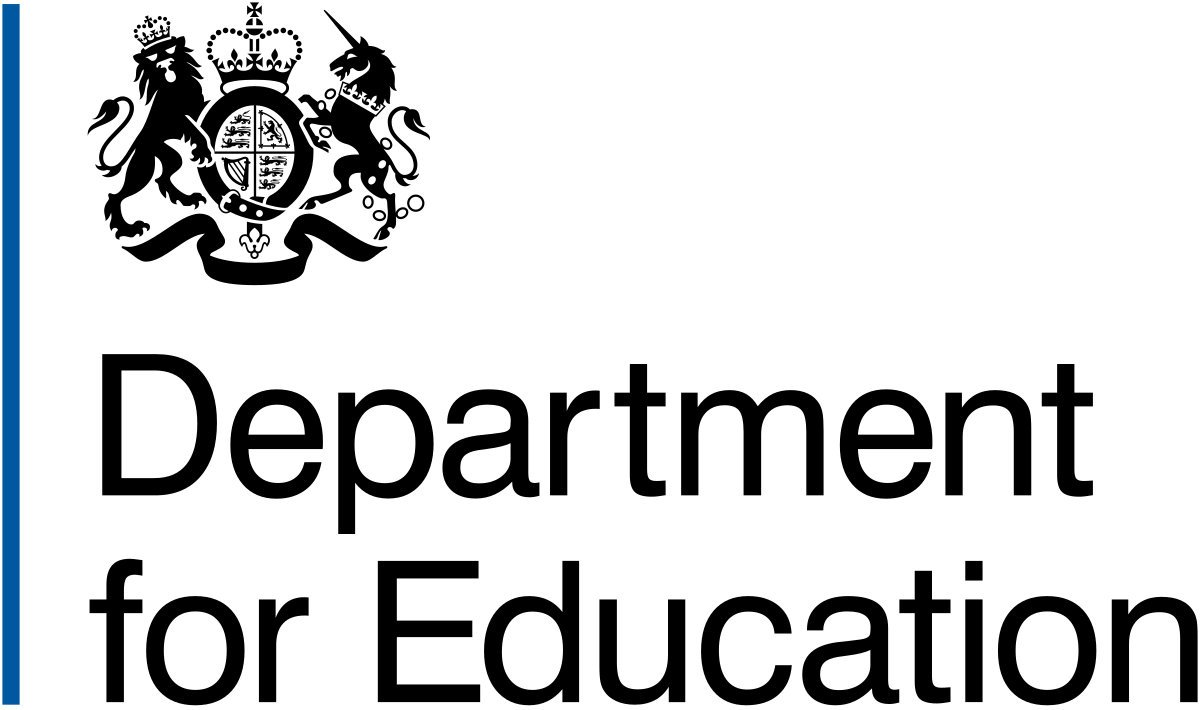
\includegraphics{images/Department_for_Education.png}}
\vspace*{\fill}
\color{black}

© Crown copyright 2022

This publication (not including logos) is licensed under the terms of
the Open Government Licence v3.0 except where otherwise stated. Where we
have identified any third party copyright information you will need to
obtain permission from the copyright holders concerned.

To view this licence:

\begin{tabular}{p{0.02\linewidth} p{0.1\linewidth} p{0.88\linewidth}}
& visit & www.nationalarchives.gov.uk/doc/open-government-licence/version/3 \\
& email & psi@nationalarchives.gsi.gov.uk \\
& write to & Information Policy Team, The National Archives, Kew, London, TW9 4DU \\
\end{tabular}

About this publication:

\begin{tabular}{p{0.02\linewidth} p{0.1\linewidth} p{0.88\linewidth}}
& enquiries & www.education.gov.uk/contactus \\
& download & www.gov.uk/government/publications \\
\end{tabular}

\begin{tabular}[t]{p{0.06\linewidth} p{0.24\linewidth} p{0.04\linewidth} p{0.06\linewidth} p{0.36\linewidth}}
\raisebox{-.5\height}{
\includegraphics{images/logoTwitter.png}} &
Follow us on Twitter: @educationgovuk &
&
\raisebox{-.5\height}{
\includegraphics{images/logoFacebook.png}} &
Like us on Facebook: \qquad facebook.com/educationgovuk\\
\end{tabular}

\end{document}
